\documentclass[a4paper]{article}

%% Language and font encodings
\usepackage[english]{babel}
\usepackage[utf8x]{inputenc}
\usepackage[T1]{fontenc}

%% Sets page size and margins
\usepackage[a4paper,top=3cm,bottom=2cm,left=3cm,right=3cm,marginparwidth=1.75cm]{geometry}

%% Useful packages
\usepackage{amsmath}
\usepackage{amsfonts}
\usepackage{graphicx}
\usepackage[colorinlistoftodos]{todonotes}
\usepackage[colorlinks=true, allcolors=blue]{hyperref}
\usepackage{subfig}
\usepackage{xcolor}

\newcommand{\aw}[1]{{\color{blue} [AW: #1]}}

\title{Non-Periodic Edge States}
\author{Jonathan Michala and Alexander Pierson}

\begin{document}
\maketitle

\section{Background}
\section{Loring Index}
Given a Hamiltonian $H$ of size $2mn \times 2mn$, \aw{what is $m$, $n$?} we define equivalently sized matrices $X$ and $Y$ as such:
$$X_{ii} = \left\lfloor \frac{i-1}{2} \right\rfloor \;\text{mod}\;m, \quad\quad Y_{ii} = \left\lfloor \frac{i-1}{2m} \right\rfloor$$
with $X_{ij} = Y_{ij} = 0$ for $i \neq j$. Our aim is to find vectors that are eigenvectors \aw{this is impossible if they do not commute, also they are only diagonalizable if Hermitian, hence you are looking for vectors which are simultaneous \emph{approximate} eigenvectors of all 3 matrices} of all three of these matrices, i.e. finding $v$ such that $(X - \lambda_1)v = 0$, $(Y - \lambda_2)v = 0$, and $(H-\lambda_3)v = 0$, for real $\lambda_1,\lambda_2,\lambda_3$. This is equivalent(Annals of Physics ref) to finding near-zero eigenvalues of the matrix
$$B(X - \lambda_1, Y - \lambda_2, H - \lambda_3) =
\begin{pmatrix}
H - \lambda_3 & (X - \lambda_1) + i(Y - \lambda_2)\\
(X - \lambda_1) - i(Y - \lambda_2) & - (H - \lambda_3)
\end{pmatrix}.$$
Thus, if this matrix has an eigenvalue less than a specified norm $\epsilon$, we say that it is in the joint pseudo-spectrum of the given lattice. We can also compute the Loring index of $(\lambda_1,\lambda_2,\lambda_3)$ triples which is defined as the signature of $B$. \aw{Hastings-Loring explains the Loring index a little. The point is that } \\\\
To compute the signature of $B$ efficiently, we use the $LDL^T$ decomposition of $B$. $D$ is a block diagonal matrix with blocks of either size $1 \times 1$ or $2 \times 2$. Let $a$ and $b$ be the number of positive and negative $1 \times 1$ blocks in $D$, respectively. By J.R. Bunch, L. Kaufman (Need ref), the signature of $B$ is equivalent to the signature of $D$ which is $a - b$.
\section{Loring Index in Haldane Model}

We compute the pseudo-spectrum and Loring index on the Haldane model lattice with complex hopping and see that in the topological case, the Loring index behave much like the Chern number: on a lattice with edges, the index is $+1$ on the interior and transitions to 0 across the edge; on a periodic lattice, the index is $+1$ everywhere. In the trivial case we see a Loring index of 0 everywhere on edged and periodic lattices, which is analogous to the Chern number. This is shown in Figure \ref{fig:Loring Haldane}.
\begin{figure}
\centering
\subfloat{{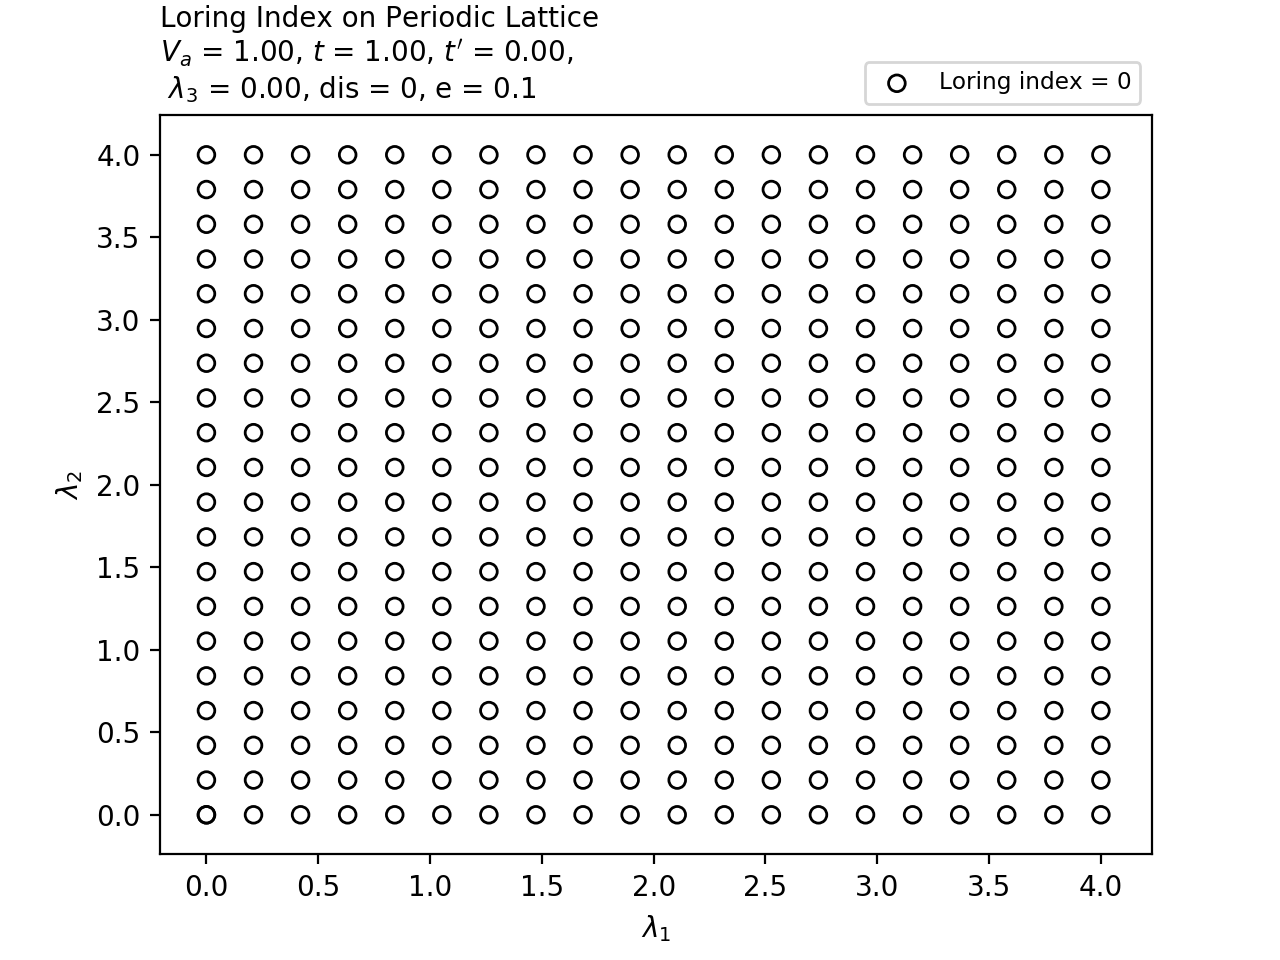
\includegraphics[width=.45\linewidth]{figures/periodic_triv} }}%
\subfloat{{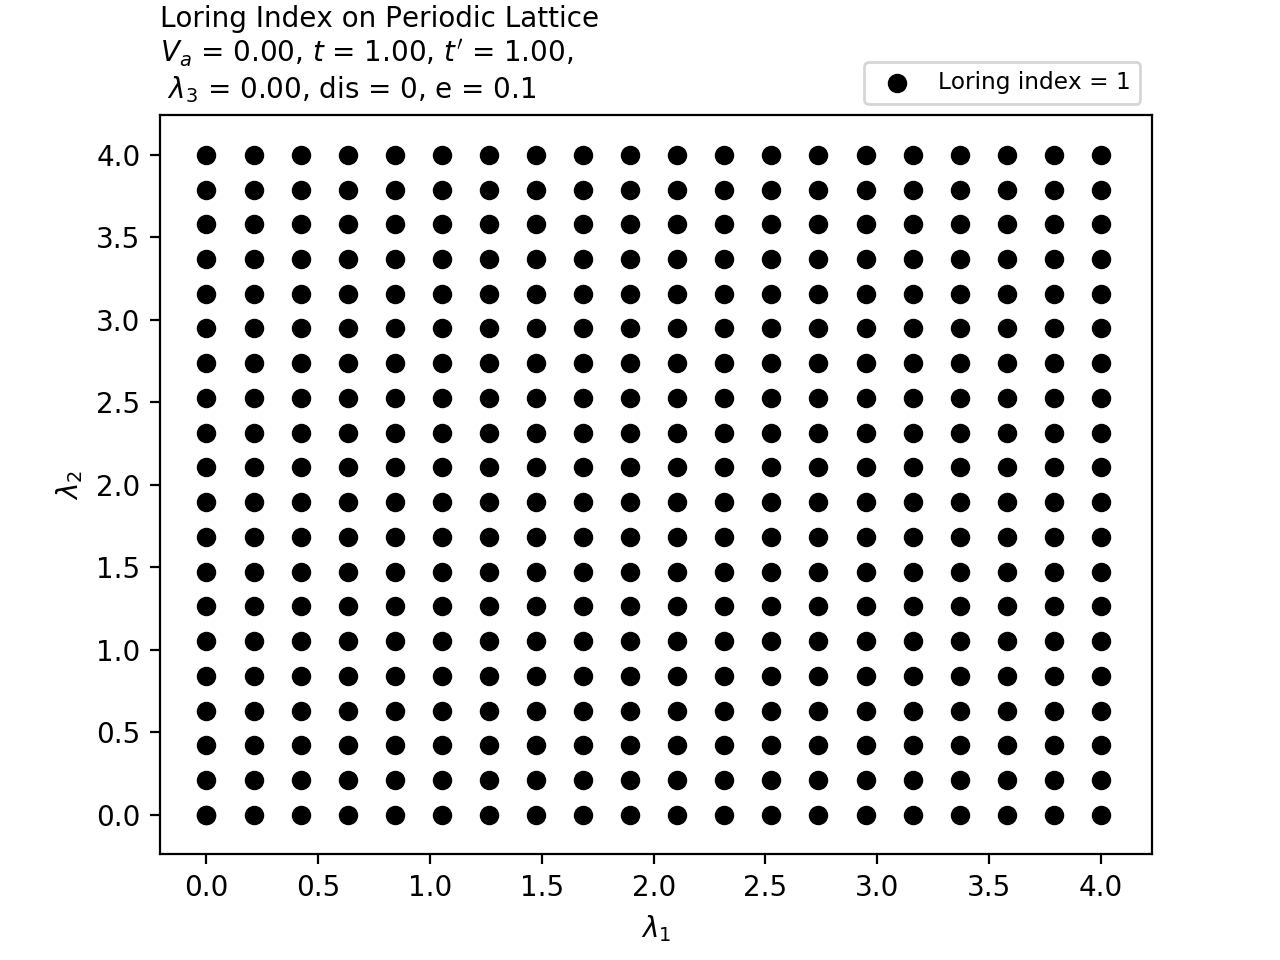
\includegraphics[width=.45\linewidth]{figures/periodic_top} }}%

\subfloat{{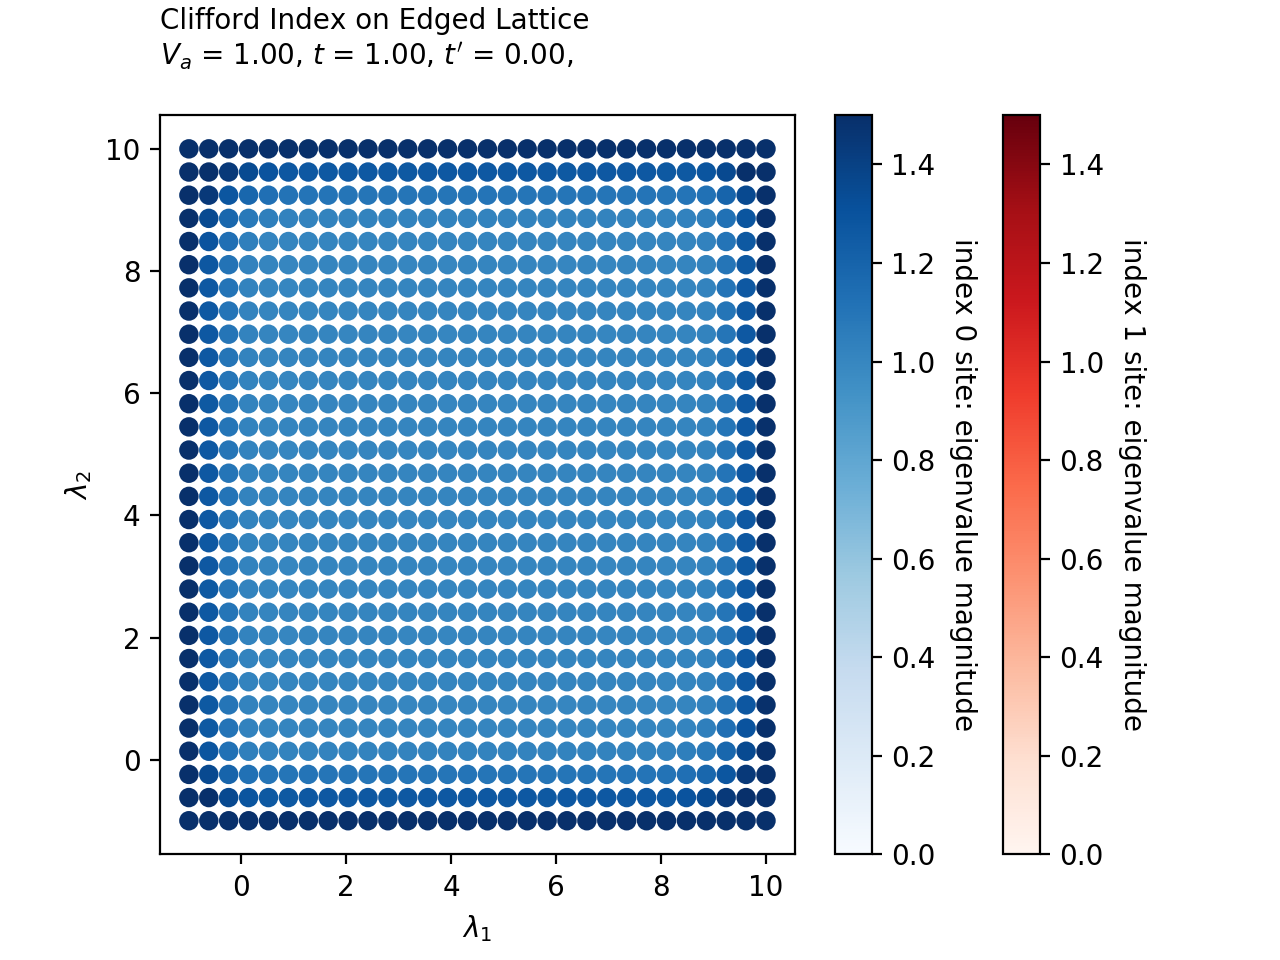
\includegraphics[width =.45\linewidth]{figures/edged_triv} }}%
\subfloat{{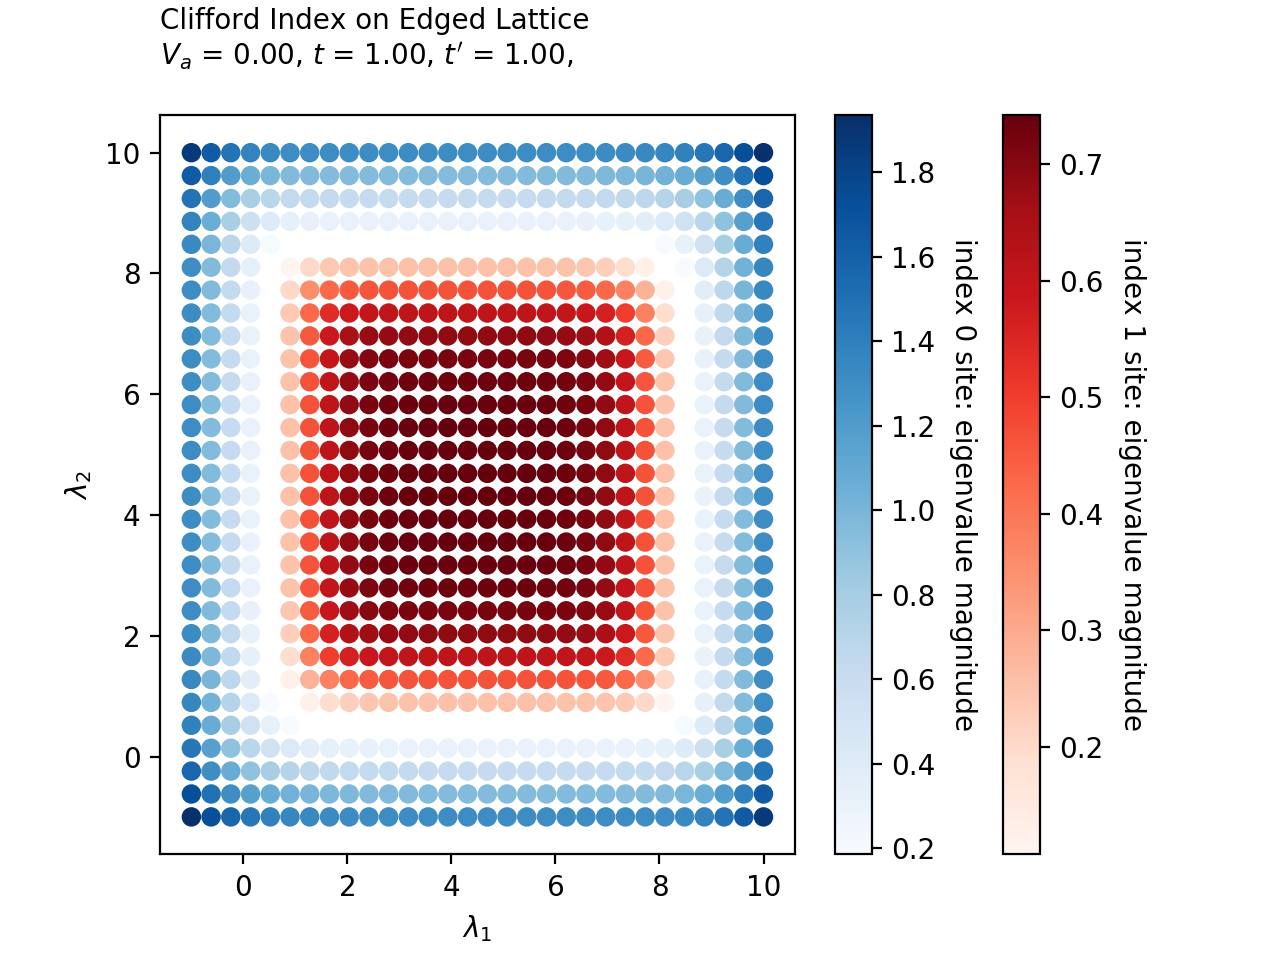
\includegraphics[width =.45\linewidth]{figures/edged_top} }}%
\caption{The top left is a trivial, periodic lattice; the top right is a topological, periodic lattice; the bottom left is a trivial, edged lattice; and the bottom right is a topological, edged lattice. Each site in these figures represents a $(\lambda_1,\lambda_2,\lambda_3)$ triple with $\lambda_3 = 0$. If a site is red, then it is in the pseudo-spectrum, i.e. $B(X - \lambda_1, Y - \lambda_2, H - \lambda_3)$ has a near-zero eigenvalue. If a site is not in the pseudo-spectrum, then it is colored black for Loring index 1 and white for Loring index 0, where the Loring index is defined as the signature of $B$.\\
}%
\label{fig:Loring Haldane}%
\end{figure}
The advantage of the Loring index compared to the Chern number is that the Chern number can only be defined on a periodic structure, whereas the Loring index can be computed on non-periodic media. We will use this advantage to study the robustness of waves on non-periodic media.

\section{Propagation in Haldane Model}
As expected, we find that localized waves propagate along the boundary of the edged, topological lattice since this is a boundary between Loring index 0 and Loring index 1.


\section{\texorpdfstring{$p_x + ip_y$}{px + ipy} Model}
\section{Loring Index in \texorpdfstring{$p_x + ip_y$}{px + ipy} Model}
\section{Propagation in \texorpdfstring{$p_x + ip_y$}{px + ipy} Model}
\end{document}